\documentclass[sigconf,review]{acmart}

\AtBeginDocument{%
  \providecommand\BibTeX{{%
    \normalfont B\kern-0.5em{\scshape i\kern-0.25em b}\kern-0.8em\TeX}}}

\usepackage[utf8]{inputenc}
\usepackage[T1]{fontenc}
\usepackage{amsmath,amssymb,amsfonts}
\usepackage{algorithmic}
\usepackage{graphicx}
\usepackage{textcomp}
\usepackage{booktabs}
\usepackage{framed}
\usepackage{float}
\usepackage{xcolor}
\usepackage{footnote}
\usepackage{xfrac}
\usepackage{balance}

\usepackage{array}
\newcolumntype{L}[1]{>{\raggedright\let\newline\\\arraybackslash\hspace{0pt}}m{#1}}

\usepackage{listings}

\definecolor{mygreen}{rgb}{0,0.6,0}
\definecolor{lightgreen}{rgb}{0.6,0.9,0.6}
\definecolor{lightyellow}{rgb}{0.9,0.9,0.6}
\definecolor{lightorange}{rgb}{0.9,0.8,0.6}
\definecolor{lightred}{rgb}{0.9,0.7,0.7}
\definecolor{mygray}{rgb}{0.5,0.5,0.5}
\definecolor{lightgray}{rgb}{0.8,0.8,0.8}
\definecolor{mymauve}{rgb}{0.58,0,0.82}


\usepackage{pifont}
\newcommand{\lstbg}[3][0pt]{{\fboxsep#1\colorbox{#2}{\strut #3}}}

\lstdefinestyle{CStyle} {
    language=C,
    backgroundcolor=\color{white},   % choose the background color
    basicstyle=\ttfamily\scriptsize,        % size of fonts used for the code
    breaklines=true,                 % automatic line breaking only at whitespace
    captionpos=b,                    % sets the caption-position to bottom
    commentstyle=\color{mygray}\bfseries,    % comment style
    escapeinside={\%*}{*)},          % if you want to add LaTeX within your code
    keywordstyle=\color{blue},       % keyword style
    stringstyle=\color{mymauve},     % string literal style
    frame=single,
    numbers=left,
    stepnumber=1,
    xleftmargin=2em,
    escapeinside={/*!}{!*/},
    moredelim=**[l][\color{mygreen}]{+\ },
    moredelim=*[l][\color{red}]{-\ }
}

\lstdefinestyle{PHPStyle} {
    language=PHP,
    alsolanguage=HTML,
    backgroundcolor=\color{white},   % choose the background color
    basicstyle=\ttfamily\scriptsize,        % size of fonts used for the code
    breaklines=true,                 % automatic line breaking only at whitespace
    captionpos=b,                    % sets the caption-position to bottom
    commentstyle=\color{mygray}\bfseries,    % comment style
    escapeinside={\%*}{*)},          % if you want to add LaTeX within your code
    keywordstyle=\color{blue},       % keyword style
    stringstyle=\color{mymauve},     % string literal style
    frame=single,
	numbers=left,
    stepnumber=1,
	xleftmargin=2em,
    escapeinside={/*!}{!*/},
    moredelim=**[l][\color{mygreen}]{+\ },
    moredelim=*[l][\color{red}]{-\ }
}


\newcounter{lstannotation}
\setcounter{lstannotation}{0}
\renewcommand{\thelstannotation}{\ding{\number\numexpr181+\arabic{lstannotation}}}
\newcommand{\annotation}[1]{\refstepcounter{lstannotation}\label{#1}\thelstannotation}


%
% Add comments in the text
%
\newboolean{showcomments}
\setboolean{showcomments}{true}
%\setboolean{showcomments}{false}

\ifthenelse{\boolean{showcomments}}
  {\newcommand{\nb}[3]{
  {\color{#2}\small\fbox{\bfseries\sffamily\scriptsize#1}}
  {\color{#2}\sffamily\small$\triangleright~$\textit{\small #3}$~\triangleleft$}
  }
  }
  {\newcommand{\nb}[3]{}
  }

\newcommand\Sof[1]{\nb{Sofia}{red}{#1}}
\newcommand\Luis[1]{\nb{Luis}{mygreen}{#1}}
\newcommand\Rui[1]{\nb{Rui}{blue}{#1}}

\makeatletter
\newcommand\footnoteref[1]{\protected@xdef\@thefnmark{\ref{#1}}\@footnotemark}
\makeatother

\setcopyright{acmcopyright}
\copyrightyear{2020}
\acmYear{2020}
%\acmDOI{}

\acmConference[ICPC'20]{ICPC '20: International Conference in Program Comprehension}{May 23--24, 2020}{Seoul, South Korea}
% \acmBooktitle{}
% \acmPrice{}
% \acmISBN{}

\begin{document}

\title{Fixing Vulnerabilities Hinders Maintainability}

\author{
    Anonymou(s) Author(s)
}

\renewcommand{\shortauthors}{Anon. et al.}

%%
%% The abstract is a short summary of the work to be presented in the
%% article.
\begin{abstract}
	
Security is a requirement of utmost importance to produce software with 
high quality. However, there is still a considerable amount of 
vulnerabilities being discovered and fixed, almost weekly. We suspect 
that when developers address these vulnerabilities on their codebases, 
they actually affect the maintainability of software, potentially 
introducing other vulnerabilities. This paper evaluates the impact of 
patches to improve security on the maintainability of open-source software. 
Maintainability is measured based on the Better Code Hub’s model of 10 
guidelines using a dataset including 1020 security commits. Results show 
that fixing software vulnerabilities hinders the maintainability of 
open-source software. We conclude that changes to codebases 
to fix vulnerabilities need to be performed with extra care.
	
\end{abstract}



%%
%% The code below is generated by the tool at http://dl.acm.org/ccs.cfm.
%% Please copy and paste the code instead of the example below.
%%
\begin{CCSXML}
<ccs2012>
 <concept>
  <concept_id>10010520.10010553.10010562</concept_id>
  <concept_desc>Computer systems organization~Embedded systems</concept_desc>
  <concept_significance>500</concept_significance>
 </concept>
 <concept>
  <concept_id>10010520.10010575.10010755</concept_id>
  <concept_desc>Computer systems organization~Redundancy</concept_desc>
  <concept_significance>300</concept_significance>
 </concept>
 <concept>
  <concept_id>10010520.10010553.10010554</concept_id>
  <concept_desc>Computer systems organization~Robotics</concept_desc>
  <concept_significance>100</concept_significance>
 </concept>
 <concept>
  <concept_id>10003033.10003083.10003095</concept_id>
  <concept_desc>Networks~Network reliability</concept_desc>
  <concept_significance>100</concept_significance>
 </concept>
</ccs2012>
\end{CCSXML}

\ccsdesc[500]{Computer systems organization~Embedded systems}
\ccsdesc[300]{Computer systems organization~Redundancy}
\ccsdesc{Computer systems organization~Robotics}
\ccsdesc[100]{Networks~Network reliability}


\keywords{Security, Software Maintenance, Open-Source Software}

\maketitle


\section{Introduction}
%
Software quality is important because it is ultimately related to the overall
cost of developing, extending and maintaining software applications~\cite{slaughter1998evaluating}. 
Software quality characteristics include, but are not limited to functional correctnes,
reliability, usability, maintainability, and security. Security is an 
important non-functional requirement during the development of software systems. 
However, there is still a considerable amount of zero-day vulnerabilities being
discovered, and fixed, almost weekly as disclosed by the Zero Day Initiative
website\footnote{Zero Day Initiative website available at
\url{https://www.zerodayinitiative.com/advisories/published/} (Accessed on \today{})}.
These vulnerabilities are gateways for attackers to penetrate systems and 
exploit their resources. As an example, in the last week of January $2019$, 
a severe vulnerability in Apple FaceTime was revealed\footnote{FaceTime vulnerability 
details available at \url{https://thehackernews.com/2019/01/apple-facetime-
privacy-hack.html} (Accessed on \today{})} --- the outcome of a design/logical
flaw that allowed callers to see and hear others without them picking up the call.
%
In $2011$, the International Organization for Standardization (ISO) issued an
update for software product quality ISO/IEC 25010 considering
\emph{Security} as one of the main software product quality characteristics~\cite{iso:2011}. 
However, many developers still lack the knowledge about best practices to deliver secure and high-quality software~\cite{Pothamsetty:2005:SEL:1107622.1107635, 8077802}.
Unmaintainable code is hard to test, analyze and re-use, and thus more difficult
to find vulnerabilities and defects. Therefore, writing maintainable code
supports the production of more reliable software preventing the introduction of 
faults/vulnerabilities in the code bases. ISO describes software 
maintainability as ``the degree of effectiveness and
efficiency with which a software product or system can be modified to improve
it, correct it or adapt it to changes in environment, and in requirements'' on
software quality ISO/IEC 25010~\cite{iso:2011}. Novel tools have been built to 
detect automatically software vulnerabilities (e.g., FindBugs, Infer and more). 
%
Despite these efforts, improving software security is not a trivial task and requires 
implementing refactorings that might affect software maintainability. 
Our suspiciousness is that some of the these patches may have a negative 
impact on the software maintainability and, possibly, even be the cause of the 
introduction of new vulnerabilities $-$ harming software reliability. Therefore, 
in this paper, we present an empirical study on the impact of patches of 
vulnerabilities in software maintenance accross open-source software.
%
% Software maintainability can also be defined as 
% the property of software that reveals how easily the software system can be 
% maintained~\cite{IEEEComputerSociety:2014:GSE:2616205} or recover after a failure. 
% Hedegus et al.
% ($2018$)~\cite{HEGEDUS2018313}, analyzed the difference of maintainability between
% groups of refactored elements and non-refactored and conclude that the source
% code elements subjected to refactorings had significantly lower maintainability
% than the elements not modified.
% There is still little information about the impact of patching vulnerabilities
% in open-source software maintainability. \textit{Are developers affecting software
% maintainability when trying to improve software security?}, it is what we want to
% investigate.
%
As ISO does not provide any specific guidelines or formulas to calculate 
maintainability, we resort on Software Improvement Group (SIG)'s web-based source 
code analysis service Better Code Hub (BCH) to compute the software compliance 
with a set of $10$ guidelines/metrics to produce quality software 
based in ISO/IEC 25010~\cite{Visser:2016:OREILLY}. The code metrics used by BCH 
were empirically validated in previous work~\cite{Bijlsma:2012:FIR:2317098.2317124, 8530041}. 
There are other well-known standards and models that have been proposed
to increase software security: Common Criteria~\cite{common:2009} which received
negative criticism regarding the costs associated and poor technical evaluation;
the OWASP Application Security Verification Criteria~\cite{oswap:2009} which is
focused only on web applications, and a model proposed by Xu et al. ($2013$)
~\cite{6616351} for rating software security (arguably, it was one of the
first steps taken by SIG to introduce security on their maintainability model). 
%
We use BCH's toolset to provide an assessment of maintainability in 
software mainly due to the broad number of metrics used.
From a methodological 
perspective, we leveraged a dataset of $607$ security refactorings collected from open-source 
software. We calculate software maintainability before and after the refactoring to measure its 
impact. This empirical study exhibits proof that changes 
applied in the code bases to fix vulnerabilities affect code maintainability. 
Especially, for refactorings that address \emph{Broken Authentication and Session Management} 
issues, \emph{Memory Leaks} and \emph{Denial-of-Service} attacks. This is important work
because there is still little information about the impact of security patches on the software
maintainability. With this study, 
we intend to highlight the need for tools to predict the impact of patches on 
maintainability~\cite{4724577} and documentation to help developers adopt security 
best practices~\cite{6311252, 7927935, MESQUIDA201519}.
%
%BCH compiles the ISO/IEC 25010 into a set of $10$ guidelines that are the
%base of BCH's evaluation. Two examples are the \emph{Write Simple Units of Code}
%based on the McCabe Complexity~\cite{1702388} and \emph{Keep your code base Small}
%based on the idea that smaller code bases are easier to maintain and less prone to defects~\cite{Visser:2016:OREILLY}.
%
The main contributions of the present work are:
%
\begin{itemize}
	\item An empirical study on the impact of security changes on software
	maintainability and what patterns need more attention.
	\item A replication package with all scripts and data created to perform the
	empirical evaluation, for reproducibility. Available online:
  \url{https://figshare.com/s/3e17518222df6a11a8d6}.
\end{itemize}
%
This paper is structured as follows: section~\ref{sec:motivation} introduces an
example of a security refactoring of a known vulnerability found in
OpenSSL\footnote{\label{openssl}OpenSSL is a toolkit that
contains open-source implementations of the SSL and TLS cryptographic
protocols. Repository available at \url{https://github.com/openssl/openssl}
(Accessed on \today{})}; section~\ref{sec:methodology} describes the
methodology used to answer the research questions; section~\ref{sec:results}
presents the results and section~\ref{sec:discussion} discusses their
implications; section~\ref{sec:threats}, enumerates the threats to the validity of
this study; section~\ref{sec:rw} describes the different work and existing
literature in the field of study; and, finally, section~\ref{sec:conclusions}
concludes the main findings and elaborates on future work.
%
\section{Motivation and Research Questions}\label{sec:motivation}
%
Due to time-to-market pressure and the lack of security expertise~\cite{8077802}, code-related
security flaws are generally detected \textit{after the fact}, i.e., when
hackers exploit them. It turns out that fixing these issues is as simple as
modifying the software code base. However, these refactorings may have a
negative impact on software maintenance --- e.g., developers might follow the
quickest solution to fix the problem and not necessarily the most elegant and
performant one. Thus, we want to understand how security refactorings impact
the maintainability of software. 
As an example, consider the refactoring of the Datagram Transport Layer Security
(DTLS) protocol implementation in OpenSSL\footnoteref{openssl} to address a vulnerability where an attacker could cause a Denial-of-Service
(DoS) attack by crafting DTLS handshake messages to trigger memory allocations
corresponding to large length values. This vulnerability is listed at the Common
Vulnerabilities and Exposures dictionary as CVE-$2014$-$3506$\footnote{CVE-$2014$-$3506$
details available at \url{http://cve.mitre.org/cgi-bin/cvename.cgi?name=CVE-2014-3506}
(Accessed on \today{})}. It is amongst the vulnerabilities studied in our
evaluation. The snippet, in Listing~\ref{lst:vuln}, presents the changes performed on the
\emph{ssl/d1\_both.c} file\footnote{CVE-$2014$-$3506$ fix available  at
\url{https://github.com/openssl/openssl/commit/1250f12613b61758675848f6600ebd914ccd7636}
(Accessed on \today{})} by the OpenSSL developers to patch the vulnerability. Every SSL/TLS connection begins with a handshake which is responsible by the
negotiation between the two parties. DTLS provides a mechanism for fragmenting
a handshake message over a number of packets, each of which can be transmitted
separately over the internet from one party to another. The problem in
CVE-$2014$-$3506$ is that the size of the handshake message collected by the
receiver is not verified against the maximum size allowed by DTLS. It is then
allocated to a new fragment (cf. Listing~\ref{lst:vuln}, line~36). Thus, if an
attacker has access to one of these packages, he can change the
handshake message size and trigger unnecessary memory allocations of large
length which can lead to memory exhaustion that could end in a DoS attack.
\medskip
\setcounter{lstannotation}{0}
\begin{lstlisting}[style={CStyle}, caption={Fix provided by OpenSSL developers to the
\\CVE-$2014$-$3506$ vulnerability},label={lst:vuln}]
+ static unsigned long dtls1_max_handshake_message_len(const SSL *s){ /*!\annotation{lst:func1}!*/
+  unsigned long max_len = DTLS1_HM_HEADER_LENGTH + SSL3_RT_MAX_ENCRYPTED_LENGTH;
+  if(max_len < (unsigned long)s->max_cert_list)
+     return s->max_cert_list;
+  return max_len;
+ }

  static int dtls1_reassemble_fragment(
     SSL *s, struct hm_header_st* msg_hdr, int *ok){

// [snip]

- unsigned long frag_len = msg_hdr->frag_len, max_len;
- if((msg_hdr->frag_off+frag_len) > msg_hdr->msg_len)
-    goto err;

- if(DTLS1_HM_HEADER_LENGTH +
-    	SSL3_RT_MAX_ENCRYPTED_LENGTH < s->max_cert_list)
-    max_len = s->max_cert_list;
- else
-    max_len = DTLS1_HM_HEADER_LENGTH +
-   		SSL3_RT_MAX_ENCRYPTED_LENGTH;

+ unsigned long frag_len = msg_hdr->frag_len;

- if((msg_hdr->frag_off+frag_len) > max_len)
+ if((msg_hdr->frag_off+frag_len) > msg_hdr->msg_len ||
+ msg_hdr->msg_len > dtls1_max_handshake_message_len(s))
     goto err; /*!\annotation{lst:func5}!*/

  memset(seq64be,0,sizeof(seq64be));
  seq64be[6] = (unsigned char) (msg_hdr->seq>>8);
  seq64be[7] = (unsigned char) msg_hdr->seq;
  item = pqueue_find(s->d1->buffered_messages, seq64be);
  if(item == NULL){
     frag = dtls1_hm_fragment_new(msg_hdr->msg_len, 1);

// [snip]

 static int dtls1_process_out_of_seq_message(
     SSL *s, struct hm_header_st* msg_hdr, int *ok){

// [snip]

+ if(frag_len > dtls1_max_handshake_message_len(s))
+    goto err; /*!\annotation{lst:func4}!*/

  frag = dtls1_hm_fragment_new(frag_len, 0);

\end{lstlisting}

The code changes performed to fix the vulnerability are:

~\ref{lst:func1} \texttt{dtls1\_max\_handshake\_message\_len} function was
inserted to return the maximum number of bytes allowed in a DTLS
handshake message for \texttt{s}. The minimum is $16$KB but it might be greater if
the maximum certificate list size (\texttt{s-$>$max\_cert\_list}) requires it. More
specifically, it checks if the maximum certificate list size requires more length 
than the maximum length (\texttt{max\_len}). If that condition holds, the function 
returns the size of the certificate list, otherwise, it returns the maximum length. 
This function replaces lines $17$--$21$.


~\ref{lst:func5} and~\ref{lst:func4} are guards added to different functions to
ascertain that the message and the fragment length are never higher than the
maximum allowed by DTLS. In particular, \ref{lst:func5} is responsible for patching
the vulnerability.

Although checking the maximum size of a handshake message seems an elementary
problem to repair, the example shows that there was a significant amount of
changes performed in the code base which produced a negative impact in the
maintainability. Even though the developer tries to simplify the
code base by introducing a smaller unit
\texttt{dtls1\_max\_handshake\_message\_len} (\ref{lst:func1}), this change disrupts
one of the guidelines proposed by the Software Improvement Group (SIG) for
building maintainable software~\cite{Visser:2016:OREILLY}. It adds a new branch
point to the \texttt{dtls1\_process\_out\_of\_seq\_message} unit
(\ref{lst:func5}) increasing the cyclomatic complexity and breaking the
\emph{Write Simple Units of Code} guideline which resulted in a negative impact on the
OpenSSL maintainability.

In this paper, our concern is to study whether, while improving software
security, developers are also negatively impacting the maintainability of their
software applications. To answer the following two research questions, we use a
dataset of security refactorings~\cite{Reis:2017:IJSSE} to measure the impact of
the changes in the maintainability of open-source software.

\begin{framed}
\textit{\textbf{RQ1} What is the impact of security refactorings on the
maintainability of open-source software?}
\end{framed}
\vspace{-0.1cm}

Often security flaws require refactoring code to make software more secure.
However, there is no evidence yet of how security refactorings impact the
maintainability of open-source software. Our suspicion is that developers tend
to introduce technical debt in their software when refactoring the code base to
address a security flaw because they tend to choose the easiest path to solve
it. To address it, we compute the maintainability of $607$ commits using the
\emph{Better Code Hub} tool. The same approach is applied to a randomly generated
dataset of regular commits --- baseline --- that we use to understand how
maintainability evolves when security refactorings are performed versus when
they are not.

\begin{framed}
\textit{\textbf{RQ2} Which patterns of security refactorings are more likely to
affect open-source software maintainability?}
\end{framed}
\vspace{-0.1cm}
% here
There are security flaws that are more difficult to refactor than others. For
instance, implementing secure authentication is not as easy as fixing a
cross-site scripting vulnerability since usually the last one can be fixed
without adding new lines of code. A typical fix for the cross-site scripting
vulnerability is presented in Listing~\ref{lst:fix}. The developer added the
function \texttt{htmlentities} to \textit{escape} the data given by the variable
\texttt{\$\_['file']}. Knowing which patterns are more likely to increase
maintainability issues is one step forward to bring awareness to security
engineers of what patterns need more attention. The taxonomy of security
patterns used to answer this question is the same as the one provided by the
authors of the dataset~\cite{Reis:2017:IJSSE}. Maintainability is measured
separately for each pattern.\\

\setcounter{lstannotation}{0}
\begin{lstlisting}[style={PHPStyle}, caption={Fix provided by \texttt{nextcloud/server} developers to a \\Cross-Site Scripting vulnerability},label={lst:fix}]
 <ul>
  <li class='error'>
   <?php echo $l->t('Cloud not found');?>
   <p class='hint'>
    <?php
-   if(isset($_['file'])) echo $_['file']
    ?>
   </p>
   <p class='hint'>
    <?php
+   if(isset($_['file'])) echo htmlentities($_['file'])
    ?>
   </p>
  </li>
 </ul>

\end{lstlisting}

\section{Methodology}\label{sec:methodology}
%
The methodology used to measure the impact of security patches on the
maintainability of open-source software is discussed in this section.
The methodology comprises the following steps, as illustrated in
Figure~\ref{fig:met}:

\begin{enumerate}
	\item Combine the datasets from related work that classifies
the activities of developers addressing security-oriented patches~\cite{Reis:2017:IJSSE, 10.1109/MSR.2019.00064}.
	\item
	Extract relevant data (e.g., sha, sha of the parent commit, owner of the project, name of 
	the repository) and code bases from the combined dataset containing $1335$ security
	refactorings collected from open-source software available on
	GitHub.
	\item A baseline of regular commits was randomly collected from the list of
	projects of the final dataset to evaluate the impact of regular commits on the
	maintainability of open-source software.
  \item Use the Software Improvement Group's\footnote{SIG's website: \url{https://www.sig.eu/} 
  (Accessed on \today{})} web-based source code analysis
  service \emph{Better Code Hub} (BCH)\footnote{BCH's website:
  \url{https://bettercodehub.com/} (Accessed on \today{})} to quantify maintainability
  for both security and regular commits. The code bases that resemble to the commits
  of our datasets are collected before the analysis performed by BCH.
  
\end{enumerate}
\vspace{-0.3cm}

%
\begin{figure}[h]
 	\centering 	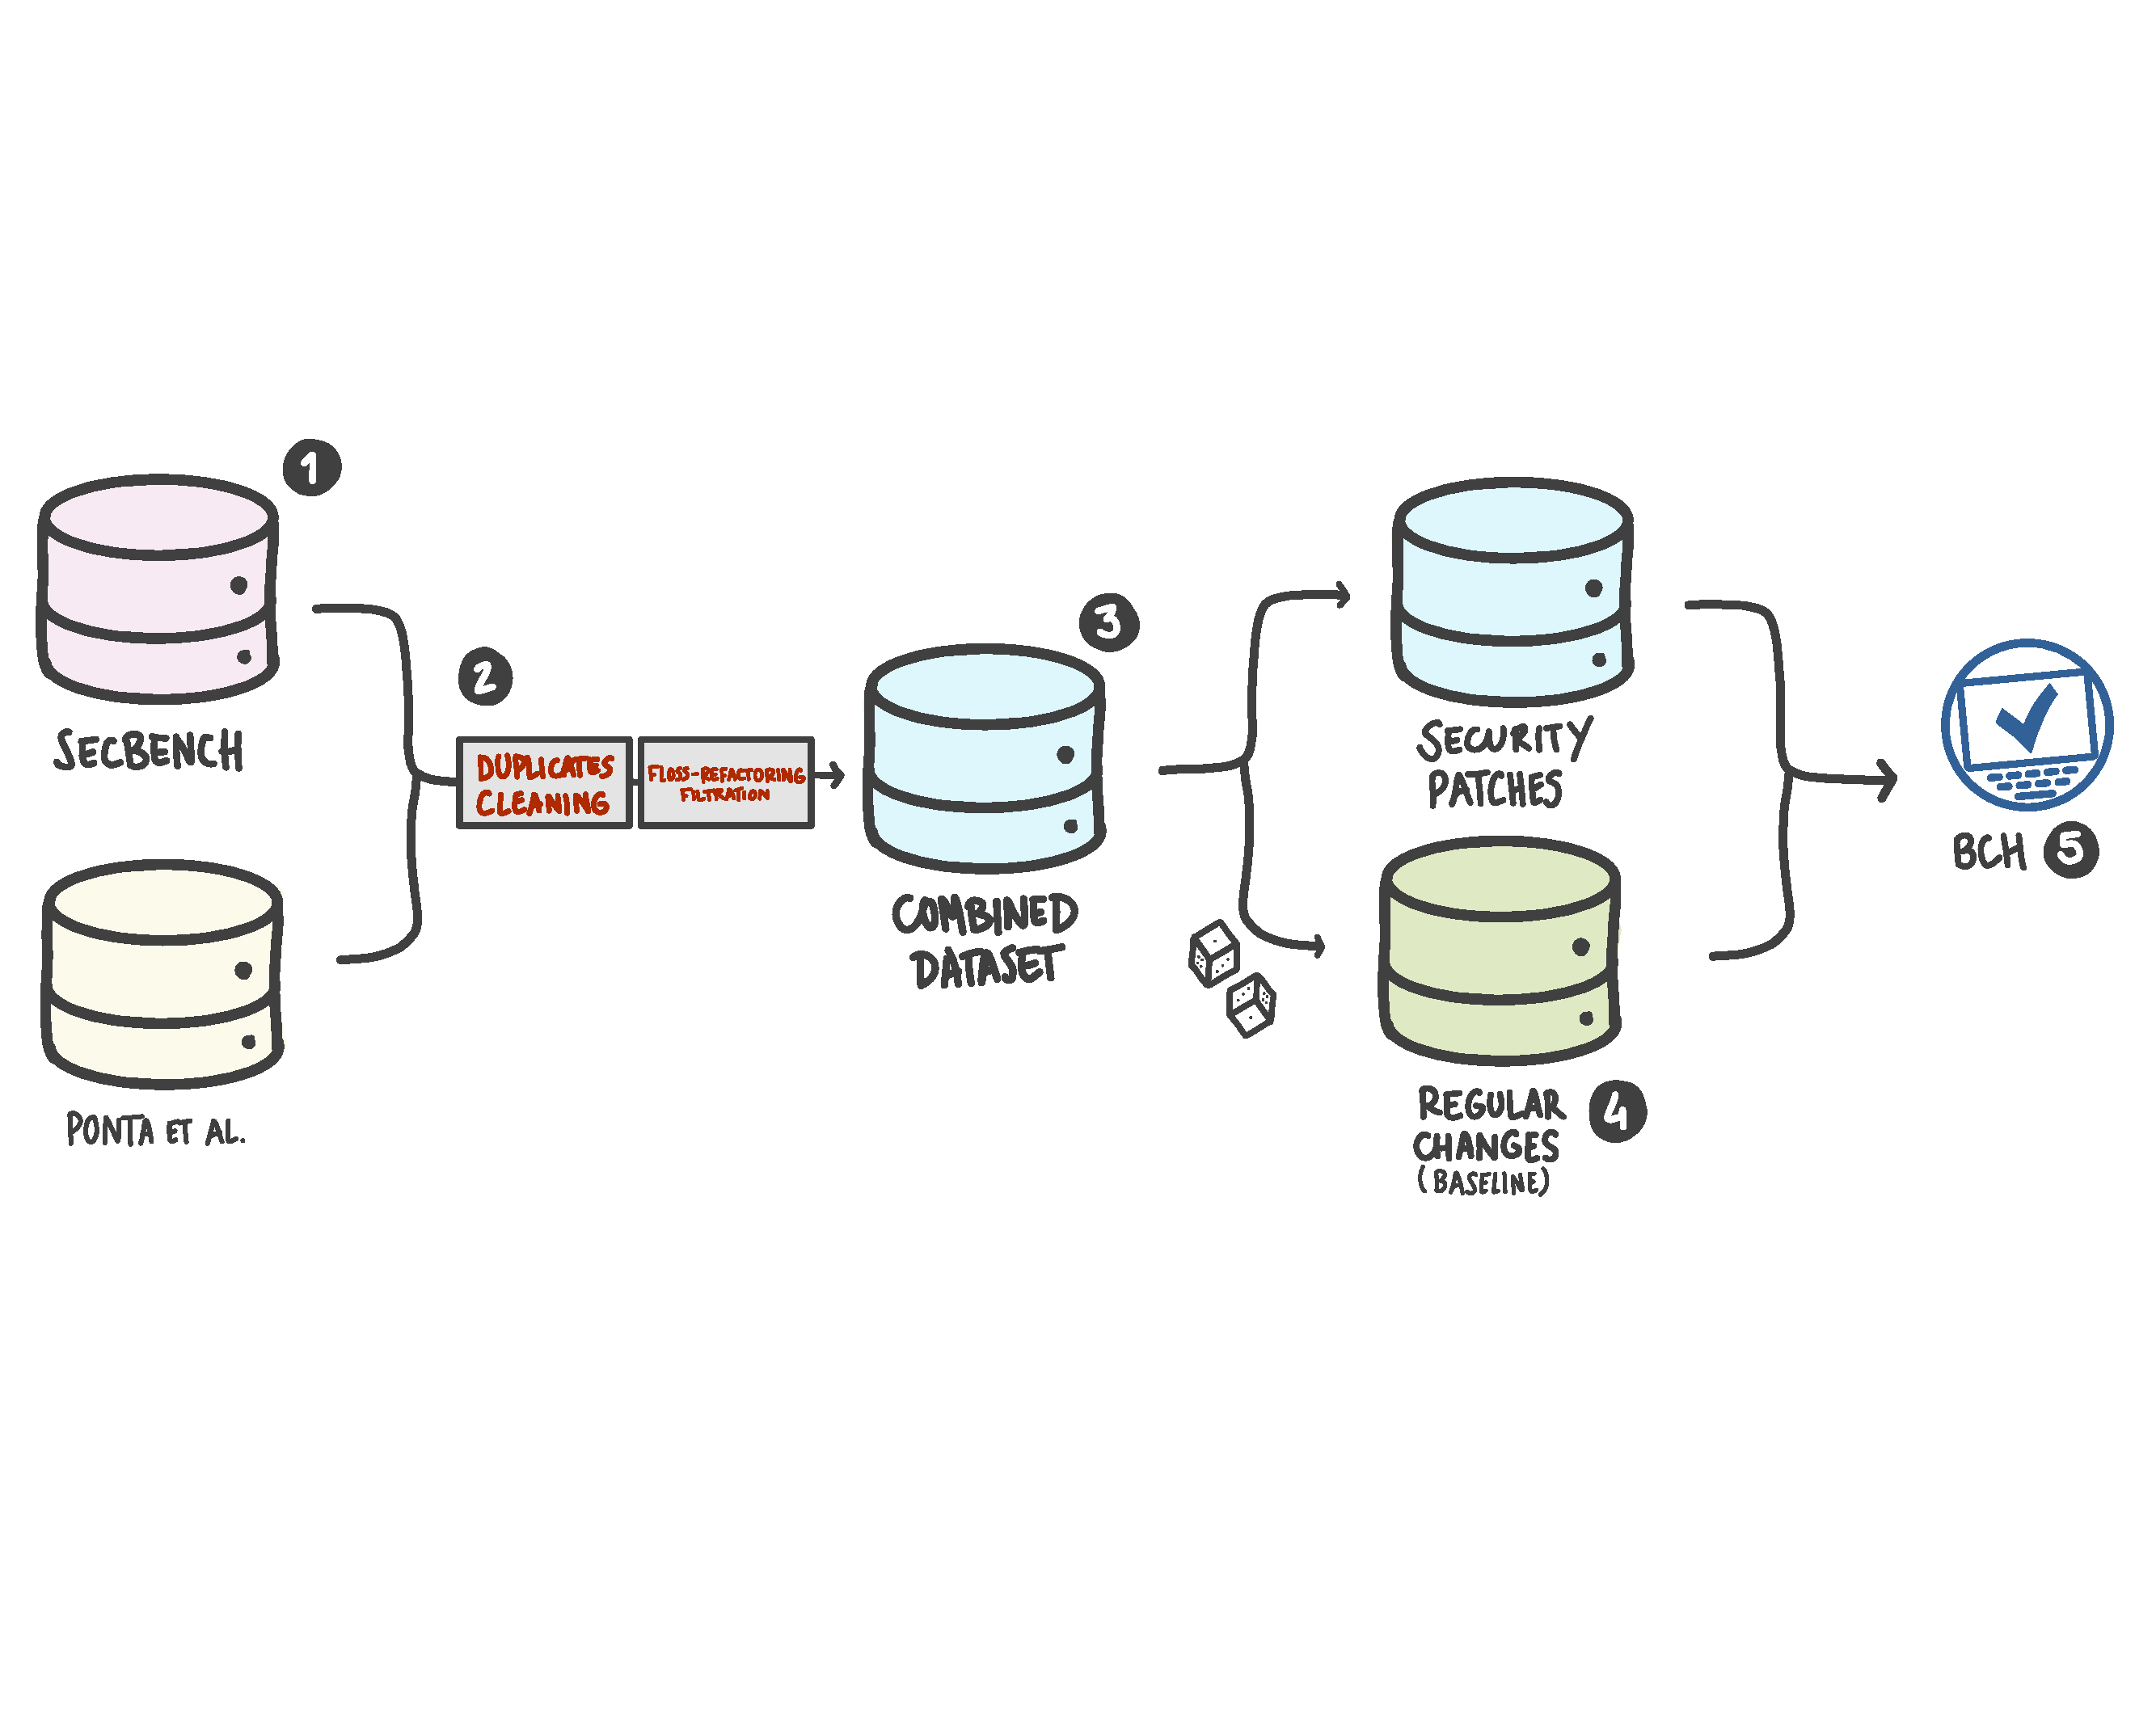
\includegraphics[width=0.4\textwidth]{figures/methodology.pdf}
 	\caption{Study Methodology\Sof{Needs to be updated. Add Vulas.}}
	\label{fig:met}
	
\end{figure}
	\vspace{-0.2cm}

%
\subsection{Datasets}
%
To evaluate the impact of security refactorings on the maintainability of
open-source software, we use a combined dataset of security vulnerabilities which is 
the outcome of mining/manually inspect $267$ GitHub projects. Reis and Abreu 
($2017$) mined open-source
software aiming at the extraction of real examples --- created by real
developers --- to test and assess the performance of static analysis tools~\cite{Reis:2017:IJSSE} since
using hand-seeded test cases or mutations could lead to misleading assessments
of the capabilities of the tools~\cite{just2014mutants}. The study yielded a
dataset of $711$ test cases for $16$ security patterns. Some of the patterns
are based in the OWASP Top $10$ of $2013$~\cite{oswap:2013} and OWASP Top $10$ of
$2017$~\cite{oswap:2017}. Each test case of the
dataset is a triplet: the commit before the patching, the commit responsible
for the patching, and the snippets of code that differ from one version to
another (typically, called \textit{diffs}) --- where one can easily review the
code used to fix the security flaw. In this study, we focus on computing the
maintainability of the commits before and after the security patching to
evaluate if its impact was positive, negative or none.

Ponta et al. ($2019$) tracked the \url{pivotal.io} website for vulnerabilities 
from $2014$ to $2019$. For each new vulnerability, the authors manually searched 
for references to commits involved in the patch on the NVD's website. However, $70\%$
of the vulnerabilities did not have any references to commits. Thus, the authors
used their expertise to locate the commits in the repositories. This technique 
yielded a database of $624$ patches~\cite{10.1109/MSR.2019.00064}. The original dataset contains $1282$ commits. One patch can have multiple commits assigned.
To fit the dataset in our methodology, we search for the first and last commits
used to patch the vulnerability. We assumed that the last commit of the patch as the fix (\emph{sha}) and the parent of the first commit as the vulnerable version (\emph{sha-p}).


The $1335$ patches in the dataset were run against the BCH toolset to
calculate their maintainability reports. However, there are refactorings
discarded from our study due to limitations of BCH: in particular, lack of
language support and project size. The final dataset used in this paper comprises
$1038$ security patches. $556$ of these patches are identified with Common Weakness
Enumeration IDs (CWE). The most prevailing categories are the following (categories
with less than $20$ instances were merged in a bigger category named \textit{Miscellaneous}):

% \begin{figure}[h]
%  	\centering 	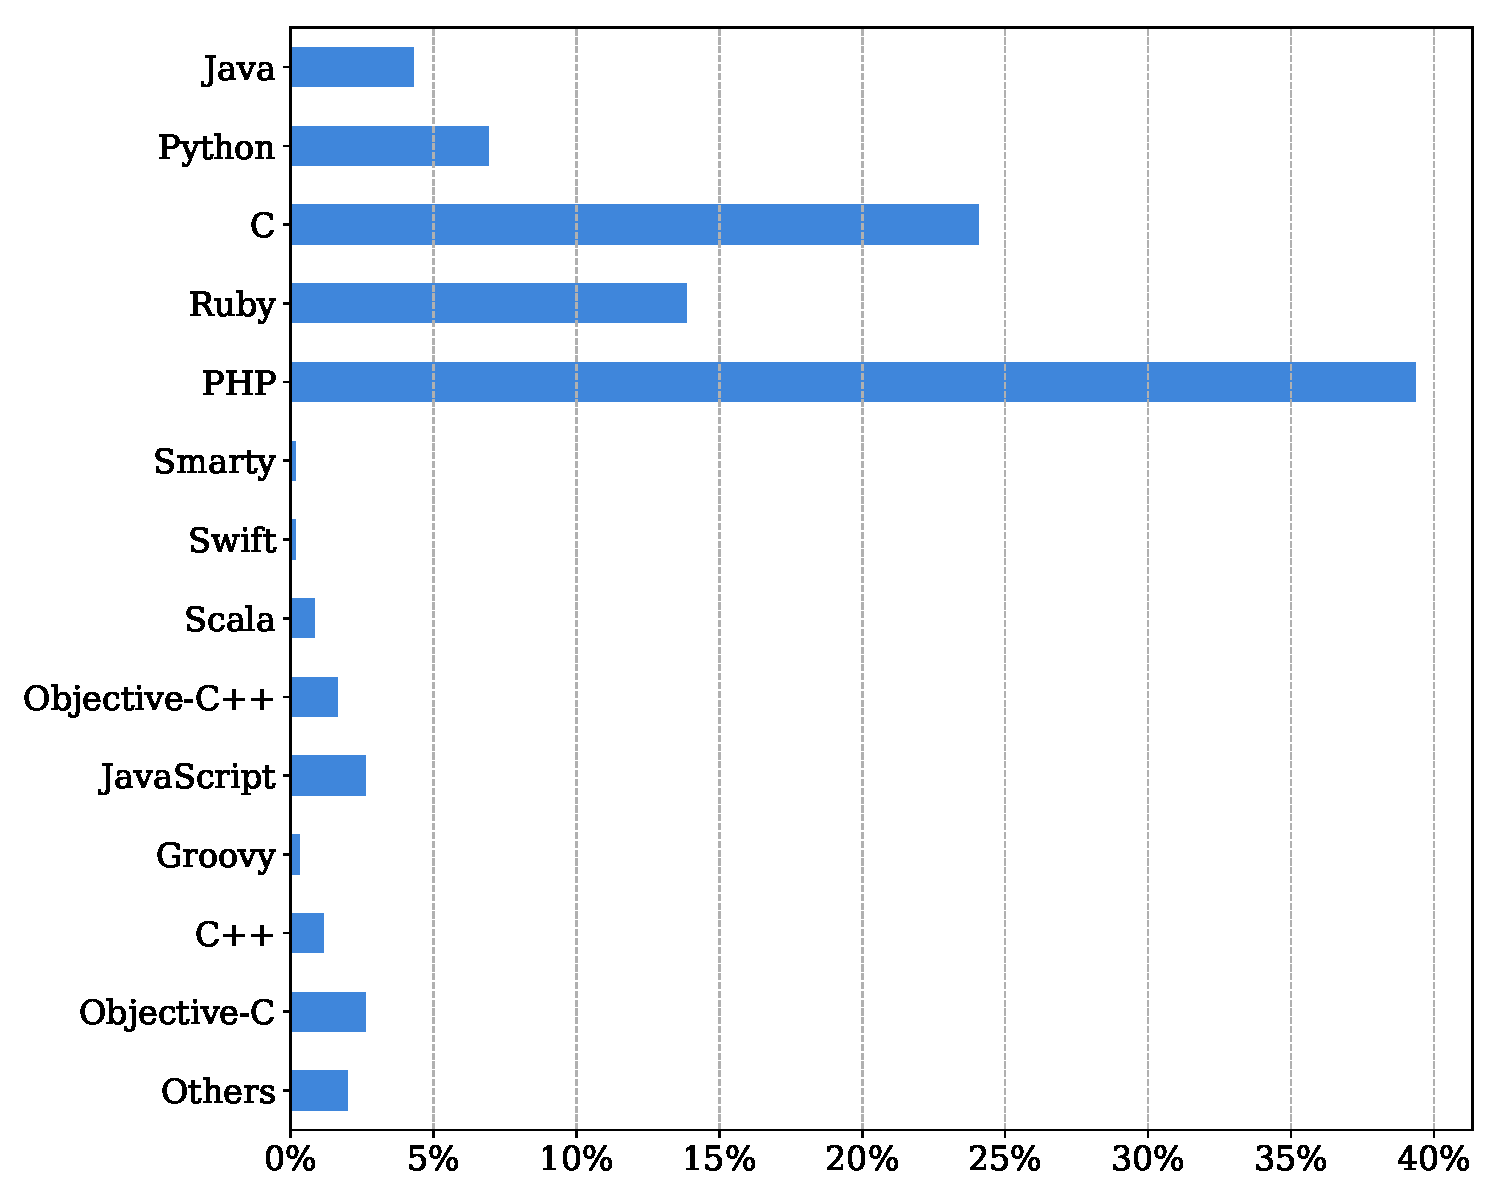
\includegraphics[width=0.5\textwidth]{figures/language_dist.pdf}
%  	\caption{Distribution of Security Refactorings per Language}
% 	\label{fig:lang}
% \end{figure}
% \vspace{-0.2cm}
%
% \begin{figure}[h]
%  	\centering 	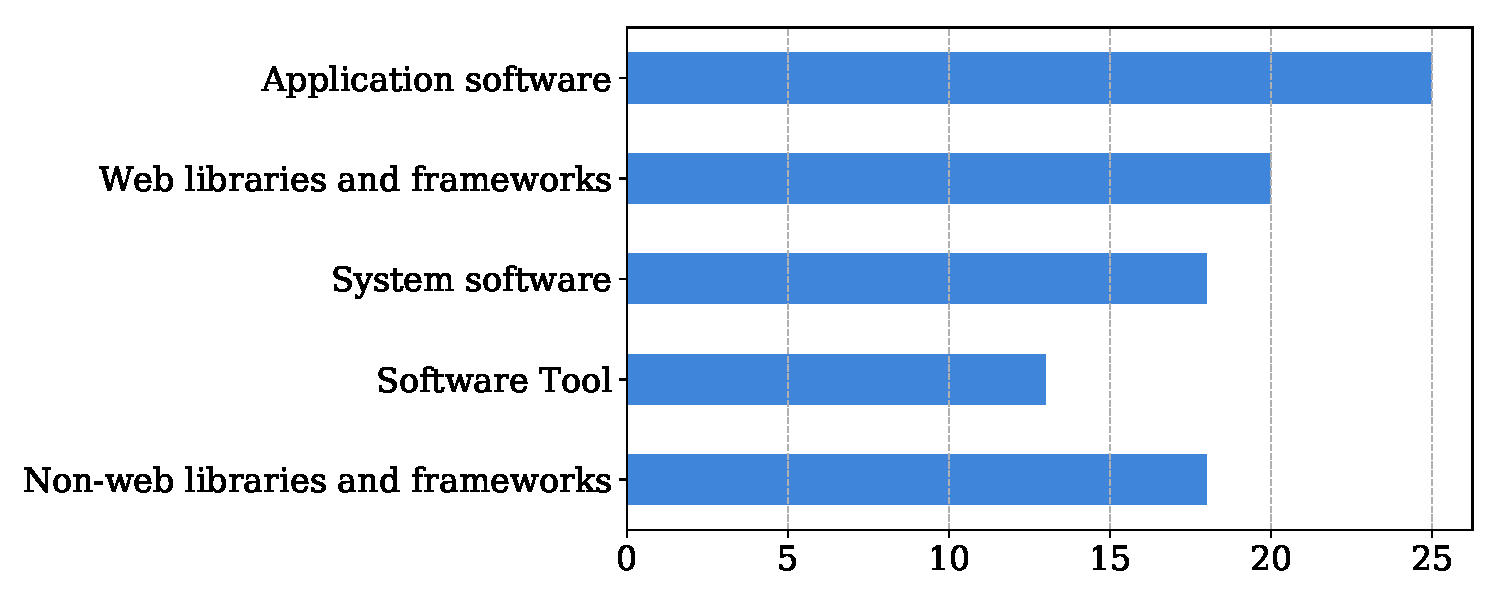
\includegraphics[width=0.5\textwidth]{figures/type_dist.pdf}
%  	\caption{Distribution of the Domain of Projects}
% 	\label{fig:domain}
% \end{figure}


\begin{itemize}
    \item \textbf{CW-89: Improper Neutralization of Special Elements used in an SQL Command/SQL Injection (23 cases).} When developers do not keep untrusted data
    separate from SQL queries. If an attacker sends a command that
    exploits the syntax of the SQL interpreter, then SQL injection attack is possible.

    \item \textbf{CWE-611: Improper Restriction of XML External Entity Reference (24 cases).} 
	XML documents are exchanged through the web containing entities with URIs
	that resolve to local/external files. Thus, when XML parsers are not well configured, 
	attackers have allowed to directly those files.
	
    \item \textbf{CWE-20: Improper Input Validation (76 cases).} When developers
	forget to validate the inputs of an application, attackers may have control
	of the control/data flow of the program.
	
    \item \textbf{CWE-200: Information Exposure (39 cases).} Application's logs are one way of intentional/unintentional disclosure information
	to attackers. Many times attackers get access to logs when sould not be authorized to.
	
	\item \textbf{CWE-352: Cross-Site Request Forgery/CSRF (22 cases).} Poor session tokens generation
    and management usually allow attackers to send forged HTTP requests
    including authentication information from the victim to the vulnerable web
    application.

	\item \textbf{CWE-264: Permissions, Privileges, and Access Controls (59 cases).} Incorrectly
	    implemented functionalities related to authentication and session
	    management, allowing an attacker to gain access to session tokens,
	    passwords, keys, and other sensitive data.
	
	\item \textbf{CWE-399: Resource Management Errors (22 cases).} Resource management issues are found more frequently
		in programming languages that do not manage memory automatically (e.g., C/C++
	    and Objective-C), i.e., where developers are responsible for
	    handling it instead. It is one of the main causes of DoS attacks.
	
	\item \textbf{CWE-79: Improper Neutralization of Input During Web Page Generation/Cross-site Scripting (62 cases)} Lack of proper validation or escaping
	    allows attackers to submit untrusted data to web browsers through malicious
	    scripts that can hijack the user sessions or redirect the user to malicious
	    sites.
	
	\item \textbf{CWE-22: Improper Limitation of a Pathname to a Restricted Directory/Path Traversal (37 cases).}  When developers forget to neutralize special elements within the pathnames to files/directories, attackers 
	may leverage this flaw to resolve to a location outside of the restricted directory and gain access to documents
	or entire repositories.
	
	
	\item \textbf{Miscellaneous (674 cases)} This pattern comprises
		several other security refactorings that do not have a CWE assigned and patterns that
		do not satisfy the Wilcoxon test size requirement of more than $20$ refactorings.


\end{itemize}

% \begin{table*}[h]
% 	\centering
% 	\caption{Descriptive statistics of the projects in the dataset}
% \begin{tabular}{@{}rrrrrrrrrrr@{}}
% \toprule
%       & Forks   & Stars   & Watchers & Contributors & Commits  & Branches & Releases & Size      & Issues & Pull Requests  \\ \midrule
% mean  & 1763 & 5448 & 401   & 153       & 14834 & 45    & 129   & 122973 & 3768   & 1941 \\
% std   & 2434 & 6215 & 486   & 123       & 22234 & 150   & 189   & 209732 & 5933   & 3603 \\
% min   & 1       & 3       & 1        & 0            & 103      & 1        & 0        & 108       & 0         & 0       \\
% 25\%  & 391  & 1581    & 117   & 49           & 1440  & 4        & 19       & 8466   & 313    & 143  \\
% median  & 838  & 2836 & 248      & 99           & 5504  & 9        & 59       & 37372  & 1792   & 650     \\
% 75\%  & 2155    & 6828 & 459   & 261          & 18579 & 20       & 142   & 117699 & 4087   & 1907 \\
% max   & 16366   & 31841   & 3446     & 413          & 114378   & 1227     & 1114     & 995790    & 33970     & 19329   \\
% Total & 165771  & 512182  & 37729    & 14413        & 1394412  & 4246     & 12168    & 11559485  & 354283    & 182511  \\ \bottomrule
% \end{tabular}
% \vspace{-0.3cm}
% \label{tab:dataset}
% \end{table*}

% The dataset contains security flaws for more than $13$ different languages,
% being PHP ($39\%$) and C ($24\%$) the most prevalent ones (cf. Figure~\ref{fig:lang}).
% To classify the applications in the dataset, we use a taxonomy for open-source
% software from previous work~\cite{7816479}. Figure~\ref{fig:domain}
% presents the projects domain distribution: \textit{Application Software} ($25$),
% software that provides end-users with functional systems; \textit{Web libraries
% and frameworks} ($20$); \textit{System Software} ($18$), software that provides
% services and infrastructures (e.g., operating systems, servers and databases);
% \textit{Software Tool} ($13$), software that supports development (e.g.,
% programming languages, compilers, package managers, IDEs); and, \textit{Non-web
% libraries and frameworks} ($18$), for desktop and mobile software.
% %
% Table~\ref{tab:dataset} presents the descriptive statistics of the $94$
% open-source projects involved in this study, including the number of forks, the
% number of stars, the number of watchers, the number of contributors, the number
% of commits, the number of branches, the number of releases, size (cf. GitHub, it
% is the size of the whole repository, including all of its history, in
% kilobytes), the number of issues, and the number of pull requests.


%
\subsection{Security vs. Baseline Commits}
%
Previous studies attempted to measure the impact of regular refactorings on
open-source software maintainability~\cite{HEGEDUS2018313}. However, there is no
previous work focused on comparing the impact of security refactorings with
regular refactorings on maintainability.
We analyze the maintainability of regular commits (i.e., commits not related
to security fixes) and use them as a baseline.

The baseline dataset uses the security commits dataset as input.
Both datasets have the same size. For each
security commit, a commit with an approximate size is searched. Due to the complexity 
of some patches, it was not possible to find patches with the exact number of added and 
deleted lines. Our search uses the patch \emph{diff} to look for a new similar \emph{diff}. The algorithm follows the following steps:

\begin{enumerate}
\item Diff comparison between the security patch commit (\emph{sha}) and its parent(\emph{sha-p}).
\item Selects a random commit from the security patch project (\emph{sha-reg}).
\item Diff comparison between the random commit (\emph{sha-reg}) and its parent (\emph{sha-reg-p}).
\item Check if the size from the regular change has the same/approximated size to 
the security patch.
\end{enumerate}

Our approximation was calculated using an initial step of $1$. Every $10$ attempts to search for 
a change with the same \emph{diff} the step increased. Thus, if a change suffered $20$ deletions 
and $10$ additions. Then, in the first $10$ attempts, the algorithm searches for a \emph{diff} with 
deletions between $19$ and $21$ and additions between $9$ and $11$. After the $10$ first attempts, 
the algorithm increase the step for $2$ and searches for a \emph{diff} with deletions between $18$ and $22$ and additions between 
$8$ and $10$. We originate the regular commits from the security
commits to ensure that differences in maintainability are not a consequence of
characteristics of different projects.

\subsection{Maintainability Analysis}

As said before, the web-based source code analysis service \emph{Better Code
Hub} (BCH) is used to collect the maintainability reports of the refactorings of
each project. Table~\ref{tab:guidelines} presents the $10$ guidelines $-$ proposed
by BCH's authors for delivering software that is not difficult to
maintain~\cite{Visser:2016:OREILLY} $-$ and maps each guideline to the metric 
calculated by BCH. Some of theses guidelines are calculated using the metrics 
presented in~\cite{criteria:2017}. During each guideline evaluation, the tool
determines the compliance towards one guideline by establishing limits for the
percentage of code allowed to be in each of the $4$ risk severity levels
(\emph{low risk}, \emph{medium risk}, \emph{high risk}, and \emph{very high
risk}). If the project does not violate the thresholds, then it is compliant
with the guideline. \textbf{These thresholds are calibrated by BCH using their own
data/experience --- using open-source and closed software systems}. If a project is
compliant with a guideline, it means that it is at least $65\%$ better than the
software used by BCH to calculate the thresholds\footnote{Check the answer to
\emph{How can I adjust the threshold for passing/not passing a guideline?} at
\url{https://bettercodehub.com/docs/faq} (Accessed on \today{})}.

\begin{figure}[h]
 	\centering 	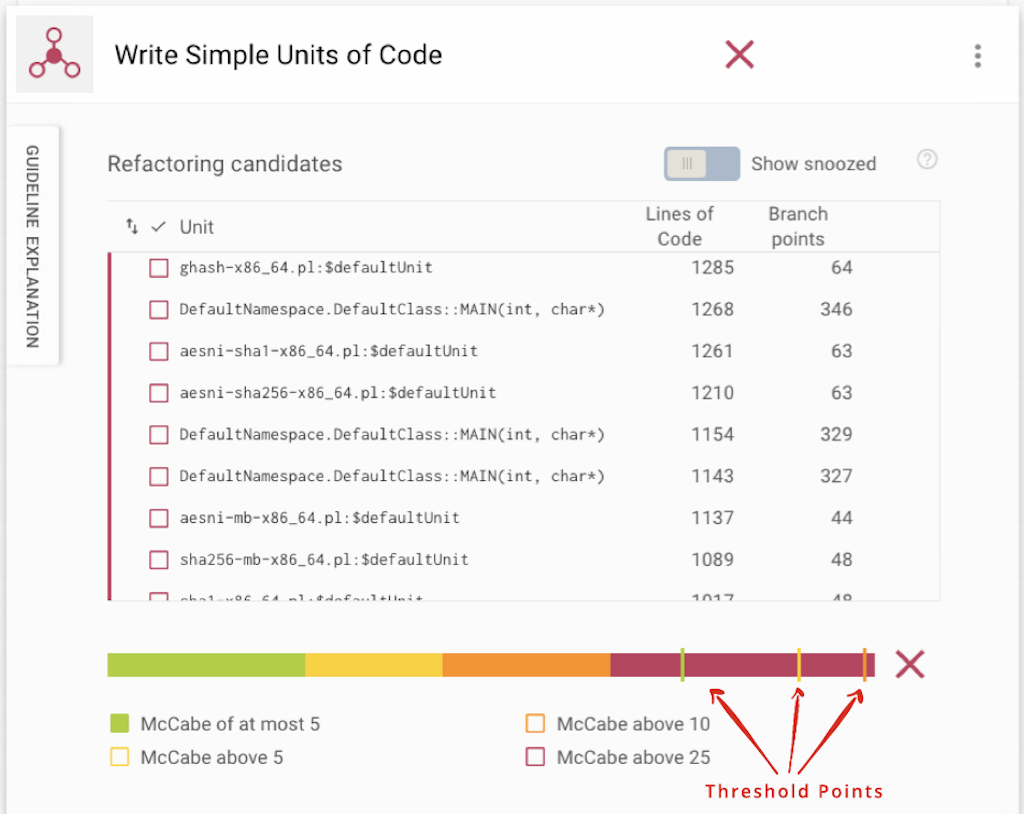
\includegraphics[width=0.45\textwidth]{figures/bch_report.png}
 	\caption{Maintainability report of OpenSSL's CVE-$2014$-$3506$ vulnerability
refactoring for the guideline \emph{Write Simple Units of Code} provided by
\emph{Better Code Hub}. This version of OpenSSL does not comply with the
guideline in the example since the bars do not reach the threshold points. This
example only complies with $\sfrac{1}{10}$ guidelines (\emph{Write Clean Code}).}
	\label{fig:bchrep}
\end{figure}

\begin{table}[H]
	\caption{Guidelines to produce maintainable code}
\begin{tabular}{L{1.66cm}L{3.25cm}L{2.65cm}}

\toprule
\textbf{10 Guidelines} & \textbf{Description} & \textbf{Metric}\\
\midrule

\textbf{Write Short Units of Code} & Limit code units to $15$ LOCs because smaller
 units are easier to understand, reuse and test them & \textbf{Unit Size:} \% of 
 LOCs within each unit~\cite{criteria:2017} \\\midrule

\textbf{Write Simple Units of Code} & Limit branch points to $4$ per unit because
it makes units easier to test and modify & \textbf{McCabe Complexity:} \# of decision 
points~\cite{1702388,criteria:2017}\\\midrule

\textbf{Write Code Once} & Do not copy code because bugs tend to replicate at
multiple places (inefficient and error-prone) & \textbf{Duplication:} \% of redundant 
LOCs~\cite{criteria:2017}\\\midrule

\textbf{Keep Unit Interfaces Small} & Limit the number of parameters to at most
$4$ because it makes units easier to understand and reuse & \textbf{Unit Interfacing:} 
\# of parameters defined in a signature of a unit~\cite{criteria:2017} \\\midrule

\textbf{Separate Concerns in Modules} & Avoid large modules because changes in
loosely coupled databases are easier to oversee and execute & \textbf{Module Coupling:} \# of
incoming dependencies~\cite{criteria:2017} \\\midrule

\textbf{Couple Architecture Components Loosely} & Minimize the amount of code
within modules that are exposed to modules in other components & \textbf{Component Independence:} 
\% of code in modules classified as hidden~\cite{criteria:2017}\\\midrule

\textbf{Keep Architecture Components Balanced} & Balancing the number of
components ease locating code and allow for isolated maintenance & \textbf{Component Balance:} 
Gini coefficient to measure the inequality of distribution between components~\cite{criteria:2017} \\\midrule

\textbf{Keep your code base Small} & Reduce and avoid the system size because
small products are easier to manage and maintain & \textbf{Volume:} \# of LOCs converted 
to man-month/man-year~\cite{criteria:2017} \\\midrule

\textbf{Automate Tests} & Test your code base because it makes development
predictable and less risky & \textbf{Testability:} Ratings aggregation $-$ unit 
complexity, component independence and volume~\cite{Visser:2016:OREILLY}
 \\\midrule

\textbf{Write Clean Code} & Avoid producing software with code smells because
it is more likely to be maintainable in the future & \textbf{Code Smells:} 
\# of Occurrences~\cite{Visser:2016:OREILLY} (e.g., magic constants and long 
identifier names) \\
\bottomrule
\end{tabular}
\label{tab:guidelines}
\end{table}


Figure~\ref{fig:bchrep} shows an example of the report
provided by BCH for a project after finishing its evaluation. The example
refers to the OpenSSL CVE-$2014$-$3506$ vulnerability refactoring ---
as described as motivating example in Section~\ref{sec:motivation}. This
version of OpenSSL only complies with $1$ out of $10$ guidelines: \emph{Write
Clean Code}.



SIG defines \emph{Units} as the smallest groups of code that can be maintained
and executed independently~\cite{Visser:2016:OREILLY} (e.g., methods and
constructors in Java). One of the guidelines with which the project does not
comply is the one presented in the report (cf. Figure~\ref{fig:bchrep}):
\emph{Write Simple Units of Code}. BCH analyzes this guideline based on the
McCabe Complexity~\cite{1702388} to calculate the number of branch points of a
method. The bar at the bottom of the figure represents the top $30$ units that
violate the guideline, sorted by severity. The violation severities are
indicated using colors, and there is a legend to help to interpret them. The
green bar represents the number of compliant branch points per unit (\emph{at
most $5$}), i.e., the number of units are compliant with ISO
$25010$~\cite{iso:2011}. Yellow, orange and red bars represent units that do not
comply with medium (\emph{above $5$}), high (\emph{above $10$}) and very high
(\emph{above $25$}) severity levels. In the bar, there are marks that pinpoint
the compliance thresholds for each severity level. If the green mark is
somewhere in the green bar it means it is compliant with a low level of
severity.

\begin{figure}[h]
 	\centering 	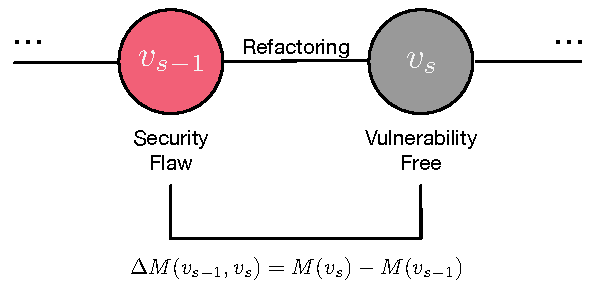
\includegraphics[width=0.75\linewidth]{figures/commit.pdf}
 	\caption{Maintainability difference for security commits}
	\label{fig:commit}
\end{figure}

Aiming to analyze the impact of security patches, we use BCH to compute the
maintainability of two different versions of the project (cf. Figure~\ref{fig:commit}):
\begin{itemize}
	\item $v_{s-1}$, the version containing the security flaw, i.e., before the
	patch (\emph{sha-p});
	\item $v_{s}$, the version free of the security flaw, i.e., after the
	patch (\emph{sha});
\end{itemize}

The BCH tool does not compute the final score that our study needs to compare
maintainability amongst different project versions. For this, we
follow previous work on measuring the impact of energy-oriented refactorings
~\cite{cruz2019energyoriented}. Luis et al. ($2019$) proposed an equation
to capture the distance between the current state of the project and
the standard thresholds calculated by the BCH based on the insights provided in ~\cite{Olivari:2018}. 
The equation considers the following:
\begin{itemize}
	\item \textbf{Size of project changes does not affect the maintainability
	difference between two versions, $\Delta M (v_{s-1},v_{s}) = M(v_{s}) - M(v_{s-1})$.} We
	aim at evaluating security patterns occurring in different projects similarly.
	Thus, the derived metric uses the \textit{raw} number of lines of code rather
  percentages for normalization purposes.
	\item \textbf{Distance to lower severity levels is less penalized than to the
	thresholds in high severity levels.} Severity level weights based on the
	severity level to count lines of code that violate maintainability guidelines.
\end{itemize}

Given the violations for the BCH guidelines, the maintainability score is computed
$M(v)$ as follows:

\begin{equation}
    M(v) = \sum_{g \in G}^{} M_{g}(v)
\end{equation}

\noindent
where $G$ is the group of maintainability guidelines from BCH
(Table~\ref{tab:guidelines}) and $v$ is the version of the software under
evaluation. $M(v) < 0$ indicates that version $v$ is violating (some of) the
guidelines, while $M(v) > 0$ indicates that version $v$ is following
the BCH guidelines. The maintenance for the guideline $g$, $M_g$ for a given version
of a project is computed as the summation of the compliance with the 
maintainability guideline for the given severity level (medium, high, and very high).
The compliance for a severity level
is calculated based on the number of lines of code that comply and not comply
with the guideline at a given severity level as explained in more
detail in previous work~\cite{cruz2019energyoriented}.  

In our analysis, we compute the difference of maintainability between the
security commit ($v_{s}$) and its parent commit ($v_{s-1}$), as illustrated in
Figure~\ref{fig:commit}. Thus, we can determine which patches had a positive, negative
or null impact on the project maintainability. 
% The compliance $C$ for a given severity
% level $l$ is derived by:
%
% \begin{equation}\label{eq:3}
%     C(l) = LOC_{compliant}(l) - w(l) * LOC_{\neg compliant}(l)
% \end{equation}
%
% \noindent
% where $LOC_{compliant}(l)$ are the lines of code that comply with the guideline
% at the given severity level $l$, $LOC_{\neg compliant}(l)$ are the lines of code
% that do not comply with the guideline at the given severity level $l$ and $w(l)$
% is the weight factor to heighten the impact of non-compliant lines in comparison to
% compliant lines. Finally, the term $w(l)$ is calculated as follows:
%
% \begin{equation}
%     w(l) = \frac{1 - \theta(l)}{\theta(l)}
% \end{equation}
%
% \noindent
% where $\theta(l)$ is the threshold in percentage of the lines of code that are
% accepted to be non-compliant with the guideline for the severity level $l$. This
% is a standard value defined by BCH. In other words, the factor $w$ is used in
% Equation~\ref{eq:3} to highlight the lines of code that are not complying with
% the guideline. Then, we compute the difference of maintainability between the
% security commit ($v_{s}$) and its parent commit ($v_{s-1}$), as illustrated in
% Figure~\ref{fig:commit}.

\subsection{Statistical Validation}\label{sec:statsval}
%
To validate the maintainability differences in different groups of commits
(e.g., baseline and security commits), we use the Paired Wilcoxon signed-rank
test with the significance level $\alpha = 0.05$~\cite{10.2307/3001968}. In
other words, we test the null hypothesis that the maintainability difference
between pairs of versions $v_{s-1}$, $v_s$ (i.e., before and after a
security-commit) come from the same distribution. Nevertheless, this test has a
limitation: it does not consider the groups of commits with a zero-difference
maintainability. In $1959$, Pratt provided an improvement to the test to solve
this issue making the test more robust. Thus, we use a version of the Wilcoxon
test that incorporates the cases where maintainability is different from zero~\cite{10.2307/2282543}.
To understand the effect-size, as
advocated by the Common-language effect sizes\cite{graw:1992}, we compute the
mean difference, the median of the difference, and the percentage of cases that
reduce maintainability.
%
\section{Results}\label{sec:results}

As mentioned before, this study evaluates $1038$ security and baseline commits
from $267$ distinct open-source projects. The following section presents the
results obtained for each research question.

\begin{framed}
\textit{\textbf{RQ1} What is the impact of security refactorings on the
maintainability of open-source software?}
\vspace{-0.1cm}
\end{framed}
\vspace{-0.1cm}

The impact of security and baseline commits in the maintainability of
open-source software is presented in Figure~\ref{fig:secvsreg}. For each type of
change, three types of impact of refactorings in the software maintainability
are presented: \emph{negative}, maintainability decreases (\emph{red});
\emph{none}, maintainability remains the same (\emph{yellow}); and,
\emph{positive}, maintainability increases (\emph{green}). Next to each
type of change, it is shown the mean ($\overline{x}$) and median (M)
of the maintainability difference and the p-value resulting from the
Paired Wilcoxon signed-rank test.


\begin{figure}[h]	
 	\centering 	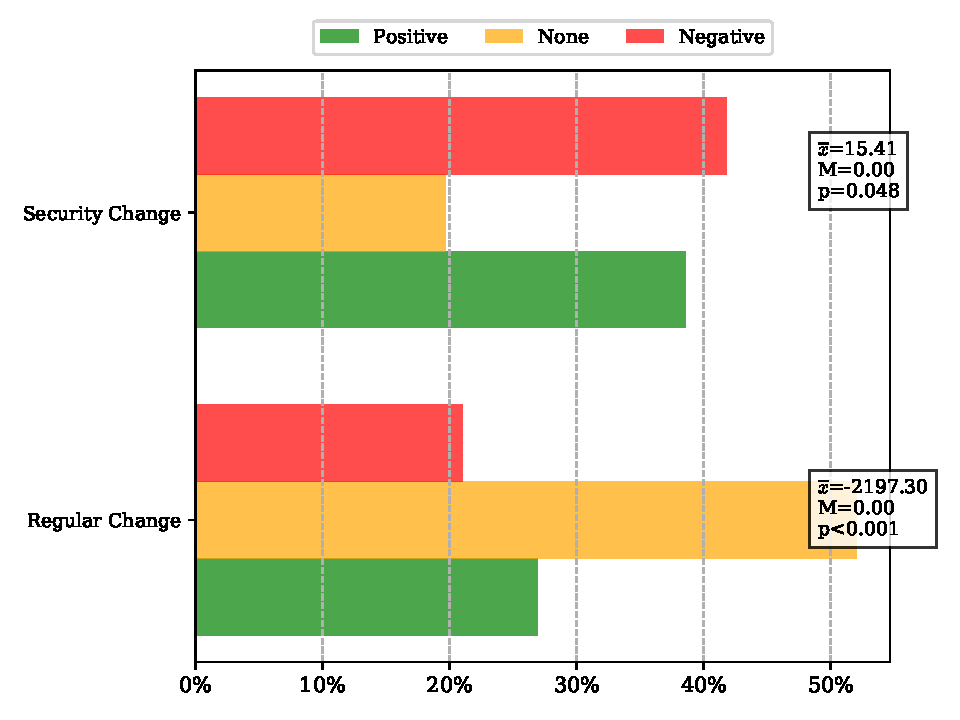
\includegraphics[width=0.46\textwidth]{figures/maintainability_sec_vs_reg.pdf}
 	\caption{Maintainability difference for security and baseline patches}
	\label{fig:secvsreg}
	
\end{figure}

\begin{figure}[h]
 	\centering
 	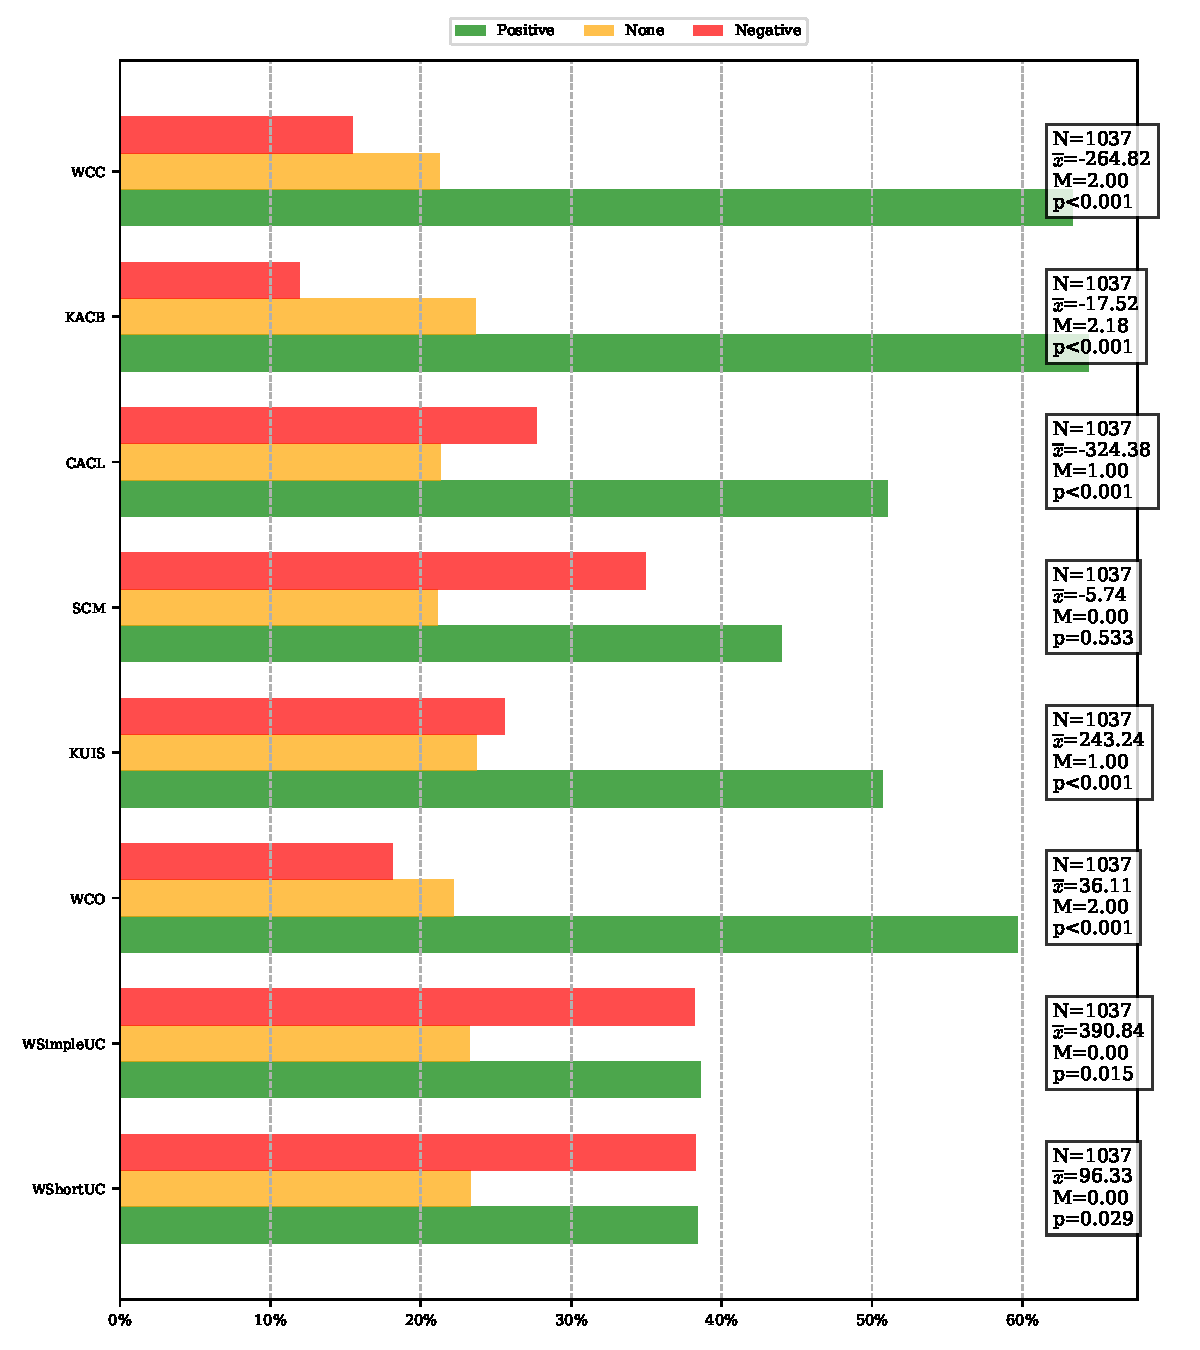
\includegraphics[width=0.57\textwidth]{figures/impact_per_guideline.pdf}
 	\caption{Impact of a security patch in 8 out of the 10 guidelines.}
	\label{fig:guidelines}
	
\end{figure}

\begin{figure}[h]
 	\centering
 	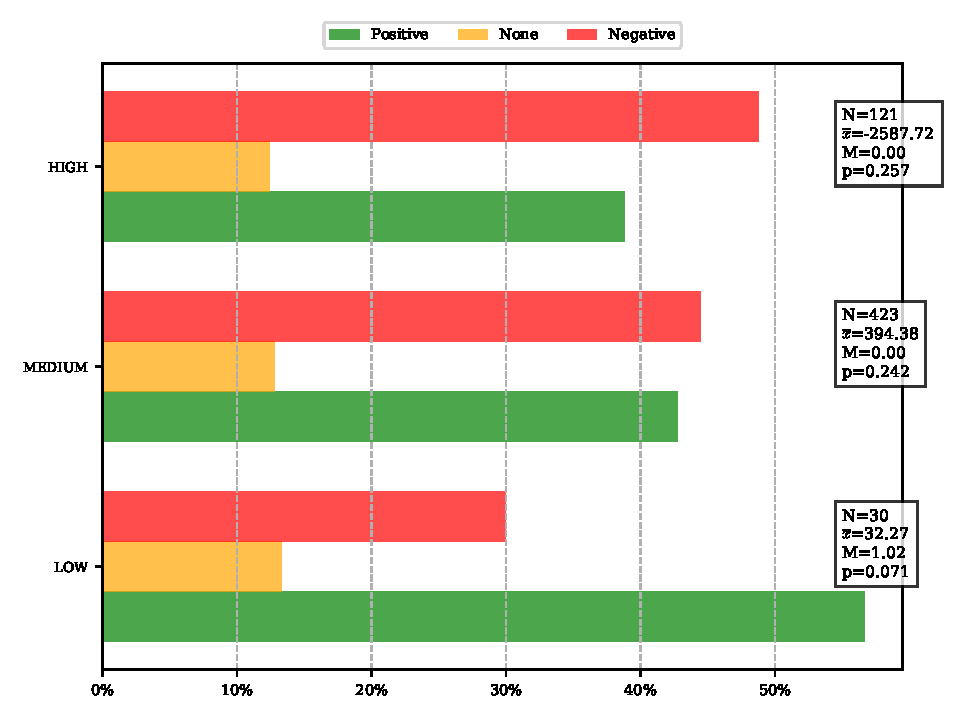
\includegraphics[width=0.5\textwidth]{figures/maintainability_severity.pdf}
 	\caption{Maintainability difference by the vulnerabilities severity.}
	\label{fig:severity}
	
\end{figure}

Regarding security commits results, we observe that maintainability decreases in
$40.20\%$ ($244$), remains the same in $30.5\%$ ($185$) and increases in $29.33\%$
($178$) of the cases after security refactorings are applied. The resulting
p-value of the Paired Wilcoxon signed-rank test is $1.21$x$10^{-10}$.
Since the p-value is below the significance level of $0.05$, we argue that
\emph{security refactorings have a negative impact in the maintainability of
open-source software}.

For regular commits, we observe that the maintainability decreases in $41.35\%$
($251$) of the cases after regular refactorings are applied. But in contrast
to security commits, it increases in $58.16\%$ ($353$) and remains the same in
$0.5\%$ ($3$) of the cases. The resulting p-value of the Paired Wilcoxon signed-rank
test is $1.54$x$10^{-6}$. Since the p-value is below the significance level of
$0.05$, we argue that \emph{regular refactorings have a
positive impact in the maintainability of open-source software}.

\begin{figure}[h]
\vspace{-0.2cm}
  \centering
  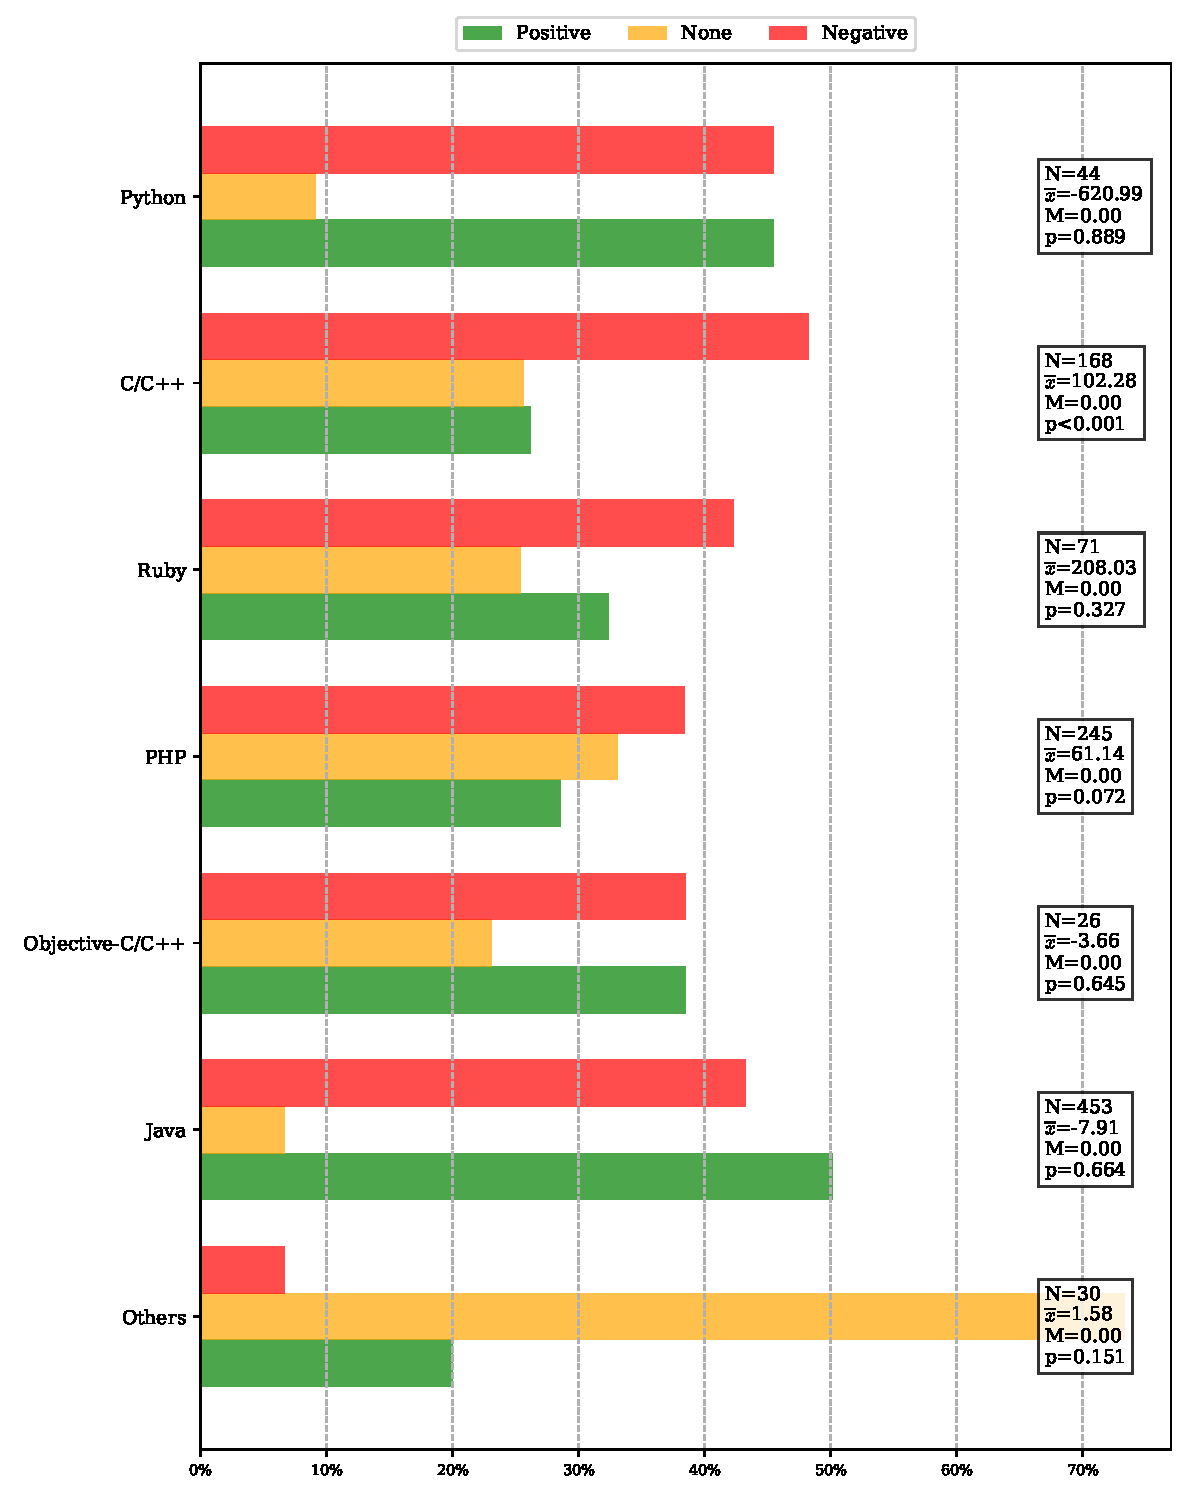
\includegraphics[width=0.5\textwidth]{figures/maintainability_language.pdf}
  \caption{Maintainability difference by language after security refactorings.}
  \label{fig:lang_main}
  
\end{figure}

We have also evaluated the impact on the maintainability per programming language
of open-source software, Figure~\ref{fig:lang_main}. Although
the dataset contains security refactorings for more than $13$ languages, we only
present the results for \emph{Java}, \emph{Python}, \emph{C}, \emph{Ruby}, and \emph{PHP}
because of the Paired Wilcoxon signed-rank test requirement: input sample has to have more 
than $20$ samples. The other languages were
integrated into \emph{Others}. The results of the Paired Wilcoxon signed-rank
test by pattern indicate that there is statistical evidence to support that the
maintainability of open-source software decreases for security refactorings in
$3$ different languages: \emph{C} (p-value = $5.72$x$10^{-9}$), Ruby (p-value = $0.057$) and
PHP (p-value = $3.54$x$10^{-6}$). Following the \textit{American Statistical Association} 
recommendations~\cite{doi:10.1080/00031305.2016.1154108}, we consider the results for 
Ruby as statistically significant because its p-value is on the borderline.
The results also exhibit statistical significance for when security refactorings 
are performed in \emph{Java} (p-value = $3.61$x$10^{-2}$). \emph{Python} and the 
languages that integrate the \emph{Others} set contain more cases where the 
maintainability increases. However, the results obtained for these patterns are 
not statistically significant.

\begin{framed}
\textit{\textbf{RQ2} Which patterns of security refactorings are more likely to
affect open-source software maintainability?}
\vspace{-0.1cm}
\end{framed}
\vspace{-0.1cm}

The impact of each type of security refactoring on the maintainability of
open-source software is presented in Figure~\ref{fig:pat}. The results of the
Paired Wilcoxon signed-rank per pattern exhibited statistical
evidence supporting that the maintainability of open-source software decreases
for $4$ different patterns: \emph{Broken Autentication} (p-value = $0.018$),
\emph{Denial-of-Service} (p-value = $0.029$), \emph{Memory Leak} (p-value = $0.009$) and
\emph{Miscellaneous} (p-value = $3.07$x$10^{-4}$). With statistical
significance, results demonstrate evidence that maintainability is not
negatively impacted when removing \emph{Components with Known Vulnerabilities}
(p-value = $7.96$x$10^{-4}$) and fixing \emph{Cross-Site Scripting
Vulnerabilities} (p-value = $0.001$). \emph{Injection} and \emph{Cross-Site
Request Forgery} produced more cases where refactorings had a negative
impact in the maintainability. However, the results obtained for these patterns
are not statistically significant.

Projects with \emph{Broken Authentication} flaws are the most affected ones by
security refactorings: $55.3\%$ ($21$) of the refactorings had a negative impact
in the maintainability while $35.0\%$ ($11$) yielded a positive impact, and only
$13.8\%$ ($6$) did not suffer any change. The results also show that fixing
\emph{Memory Leak}s affects the maintainability of $51.3\%$ ($41$) of the cases
and leaves only $13.8\%$ ($11$) of the cases unaffected. In $35\%$ ($28$) of the
cases, maintainability increased. Refactoring vulnerabilities that allow
\emph{Denial-of-Service} attacks (e.g., CVE-$2014$-$3506$) have a negative
impact of $47.5\%$ ($19$) in the maintainability of open-source software while
$30.0\%$ ($12$) of the cases exhibit maintainability improvement and $22.5\%$
($9$) show that maintainability does not suffer any change. The
\emph{Miscellaneous} refactorings pattern integrates several types of security
flaws. These type of refactorings harm maintainability in $43.1\%$ ($84$) of the
cases. In $31.8\%$ ($62$), there is no impact and for the
other $25.1\%$ ($49$) maintainability increases.

It is also important to notice that overall the maintainability of open-source
software is not affected by \emph{Cross-Site Scripting} vulnerabilities and by
\emph{Using Components with Known Vulnerabilities}. \emph{Cross-Site Scripting}
does not suffer any decrease in the maintainability of $55.3\%$ ($63$) of cases
and $21.1\%$ ($24$) have a positive effect on it. Only $23.7\%$ ($27$) of the
cases hinder the software maintainability. From the $21$ cases evaluated for
\emph{Using Componentes with Known Vulnerabilities}, only $4.8\%$ ($1$) have a
positive effect in the maintainability of software while $14.3\%$ ($3$) harms
maintainability software, and $81\%$ ($17$) have no effect in the
maintainability.


\begin{figure}[h]
 	\centering
 	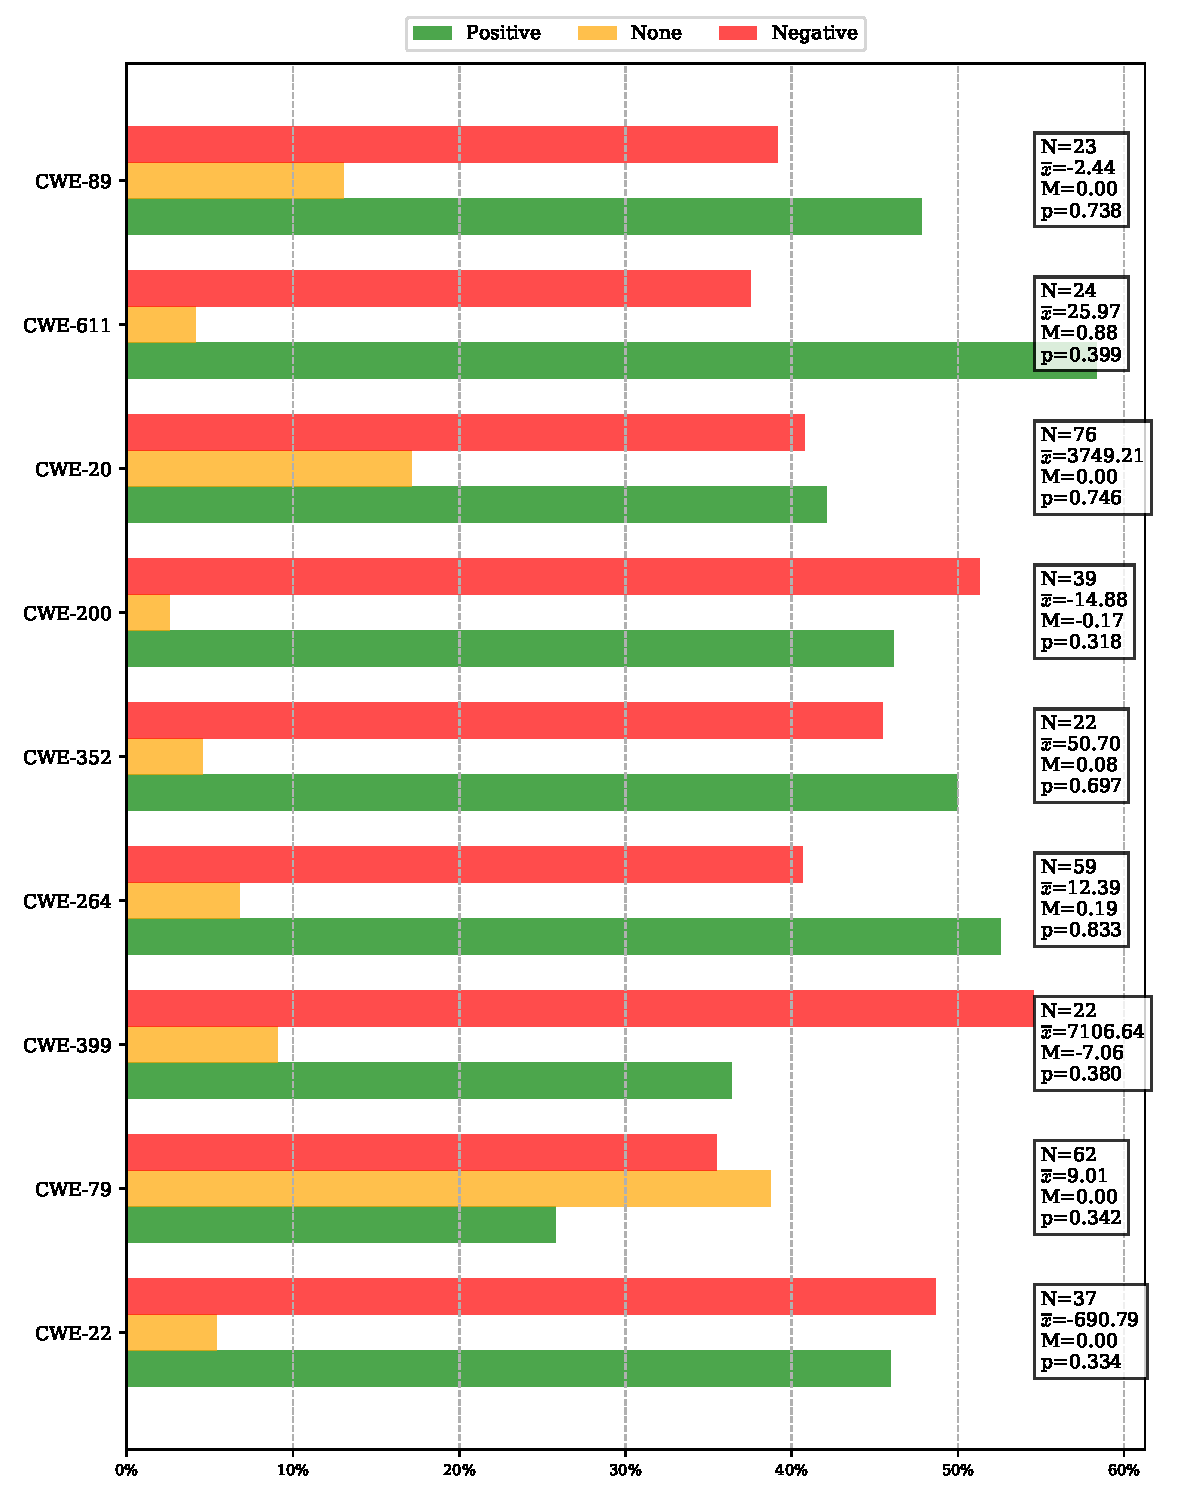
\includegraphics[width=0.5\textwidth]{figures/maintainability_cwe.pdf}
 	\caption{Maintainability difference by pattern after security patches.}
	\label{fig:pat}
	
\end{figure}



\section{Discussion}\label{sec:discussion}

In this section, we discuss the results and answer the proposed research questions.

\begin{framed}
\textit{\textbf{RQ1} What is the impact of security refactorings on the maintainability
of open-source software?}
\vspace{-0.1cm}
\end{framed}
\vspace{-0.1cm}

\textbf{\textit{Security refactorings harm the maintainability of open-source software.}}
%
We found that $40.2\%$ of the security refactoring have a negative impact on the
maintainability of open-source software (cf. Figure~\ref{fig:secvsreg}). This raises
a new tradeoff when developers need to fix vulnerabilities on their projects
because they might be affecting the software maintainability or even introducing
new vulnerabilities. This study exhibits evidence that developers may have to
reduce maintainability for the sake of security. We understand that developers
should be able to produce secure code without affecting the maintainability of
their projects. But there are still some concerns that need to be addressed:
\begin{itemize}
	\item \textbf{Documentation} of software must provide developers with the
	best practices to implement secure and maintainable software. Unmaintainable
	code is difficult to test, analyze and re-use.

	\item\textbf{Programming Languages} should provide new design patterns to
	easily implement security patterns without endangering maintainability.
	Ultimately, new programming languages, both secure and maintainable by design,
	may be designed to help developers be highly productive when writing and
	maintaining  secure applications. One example is the need for designing new
	authorization mechanisms since these are one of the most complex security
	features to implement.

	\item \textbf{Software Developers} lack the knowledge to create secure and
	maintainable code. Mainly because academic curricula are not yet prepared
	to properly educate them. Universities should do their part on making
	this possible. Online services such as BCH have also a great potential to help
	developers to be more aware of the maintainability issues introduced by their
	changes. Thus, developers can put more work into improving their code maintainability
	and avoid common issues such as code duplication.

\end{itemize}


We would expect that the negative impact of programming languages on
maintainability to be more severe, as arguably poor design of programming
languages and lack of using the best practices lead to more buggy and vulnerable
code~\cite{Ray:2017:LSP:3144574.3126905, 2019arXiv190110220B}. However,
Figure~\ref{fig:lang_main} shows that only \emph{C} has a negative impact of
more than $50\%$ on software maintainability. We suspect that these values are
the result of projects contributions policies. Nine of the top-10 of dataset projects  --- the
equivalent to $31.8\%$ of the commits ---
with more contributors have restrict contribution policies regarding code
standards. Some examples are the \texttt{laravel/framework},
\texttt{php/php-src}, \texttt{openssl/openssl} and \texttt{cakephp/cakephp}. For
instance, \texttt{laravel/framework} requires the \texttt{PSR-2
Standard}\footnote{PSR-2 Standard available at
\url{https://www.php-fig.org/psr/psr-2/} (Accessed on \today{})} that is a coding style guide for \texttt{PHP}.

\begin{framed}
\textit{\textbf{RQ2} Which patterns of security refactorings are more likely to
affect open-source software maintainability?}
\vspace{-0.1cm}
\end{framed}
\vspace{-0.1cm}

\textbf{\textit{Broken Authentication \& Session Management, Denial-of-Service
attacks, and Memory Leaks, and Miscellaneous patterns are more likely to affect
open-source software maintainability.}} Although there are a few refactorings
that harm software maintainability in the \emph{Cross-Site Scripting} and
\emph{Using Components with Known Vulnerabilities}, overall maintainability does
not suffer any changes for these patterns. For the remaining patterns,
\emph{Injection} and \emph{Cross-Site Request Forgery}, results are not
statistically significant.

The impact of a refactoring depends on its complexity, i.e., if the refactoring
adds complexity to the code base it is probably affecting the software
maintainability. One evidence of that is the fact of \emph{Cross-Site Scripting}
and \emph{Using Components with Known Vulnerabilities} refactorings endure more
cases without any impact in the maintainability. Typically, these types of
vulnerabilities do not need extra lines to be fixed, as shown in
Listing~\ref{lst:fix}. Whereas, \emph{Broken Authentication} and vulnerabilities
such as the one presented in Section~\ref{sec:motivation} responsible by Denial-of-Service
attacks are more difficult to fix (several code lines deleted and added).
Another example is the Apple authentication flaw discovered in $2017$
(CVE-$2017$-$13872$)\footnote{CVE-$2017$-$13872$ details available at
\url{https://support.apple.com/en-us/HT208315} (Accessed on \today{})}, where any user
could log in as root with an empty password. Patrick Wardle examined the cause
of the issue\footnote{\emph{Why $<$blank$>$ Gets You Root} available at
\url{https://objective-see.com/blog/blog\_0x24.html} (Accessed on \today{})} and
concluded that the flaw was due to the introduction of high cyclomatic complexity
in a method used to verify the password. In sum, \emph{Cross-Site Scripting} and
\emph{Using Components with Known Vulnerabilities} should take part of the
developers' preoccupations along with the other patterns that explicitly hinder
maintainability because despite their low complexity these are patterns that
still produce a considerable negative impact on the maintainability. Real
efforts have been made in creating and incorporating coding standards and best
practices in software production. However, security is still far from perfection
and fixing vulnerabilities might hinder software maintainability. Thus, it is
not only important to provide tool support to developers to help them apply these
patterns without harming software maintainability, but also to create and redesign
programming languages to facilitate developers improving software maintainability.


We measured the effect sizes between both distribution -- before and after
patches --- per language and security patterns using the Common Language Effect
Size~\cite{cliff:1993} method. Effect sizes are of a low-medium level.
Thus, considering the $0$ median and the low effect sizes, it is reasonable
to affirm that there is a significant effect but it might only be
recognized after a thoughtful data analysis.


\section{Threats to Validity}\label{sec:threats}
%
The following section presents the potential threats to the validity of this
study.
%
\subsection{Construct}
%
The maintainability formula was inferred based on the BCH's reports. The high
amount of different projects and backgrounds may require other
maintainability standards. However, BCH does use a representative benchmark of
closed and open-source software projects to compute the
thresholds for each maintainability guideline~\cite{Visser:2016:OREILLY, Baggen2012}.

\subsection{Internal}

The security refactorings dataset provided by the previous
work~\cite{Reis:2017:IJSSE} was collected based on the messages of GitHub
commits produced by project developers to classify the changes performed by them
to fix security flaws. This approach discards security refactorings that were
not explicit in commits messages. Baseline commits are retrieved randomly by selecting one commit from the same
project of a given security refactoring. This approach softens the differences
that may result from the characteristics of each project. However,
maintainability may still be affected by the developers' experience, coding
style and software contribution policies which is not evaluated in this study.
Furthermore, this evaluation considers that $607$ regular commits are enough to
alleviate random irregularities in the maintainability differences of the
baseline.

\subsection{External}

We use a dataset that only comprises refactorings of open-source software.
However, the methodology requires to access data that is not publicly available.
Thus, our findings may not extend to non-open source software. Different programming 
languages may require different coding practices to address software safety. The 
dataset comprises more commits in C and PHP, i.e., the dataset may not be representative 
of the population regarding programming languages. Our approach does not consider 
security refactorings in any other languages but English.

\section{Related Work}\label{sec:rw}

Many studies have investigated the relationship between refactorings and
software quality. Previous work focused on object-oriented metrics has evaluated the
impact of refactorings and exhibited proof that quantifying effectively the
impact of refactorings on maintainability may help to choose the appropriate
refactoring type~\cite{1167822}. In contrast to this work, Hegedus et
al.~\cite{HEGEDUS2018313} did not select particular metrics to assess the effect
of refactorings. Instead, statistical tests were used to find the metrics that
have the potential to change significantly after refactorings. The differences
of maintainability between groups of refactored elements and non-refactored were
analyzed. In addition, the authors concluded that the source code elements
subjected to refactorings had significantly lower maintainability than the
elements not affected. Studying the evolution of maintainability issues during
the development of Android apps, Malavolta et al. ($2018$)~\cite{8530041}
discovered that maintainability decreases over time. Palomba et al.
($2018$)~\cite{Palomba:2018:DIM:3231288.3231337} exhibits proof that code smells
should be carefully monitored by programmers since there is a high correlation
between maintainability aspects and proneness to changes and faults. The present
work uses a model proposed by BCH and focuses solely on evaluating the impact of
patching vulnerabilities on software maintainability.

Researchers investigated the relationship between design patterns and software
maintainability~\cite{10.1007/978-3-642-35267-6-18}. $300$ revisions of
\texttt{JHotDraw} were analyzed to conclude that every introduced pattern
instance improved software maintainability. However, other studies show that the
use of design patterns may introduce maintainability issues into
software~\cite{4493325}. Yskout et. al were not able to detect if the usage of design patterns has a positive impact, but concludes that developers prefer to work with the support of security patterns~\cite{8077802}. The present work studies how security patterns influence maintainability for open-source software.

There are studies that investigated the impact of programming languages on software
quality~\cite{Ray:2014:LSS:2635868.2635922,Ray:2017:LSP:3144574.3126905}. The first
study shows that some programming languages are more buggy-prone than others. However,
the authors of the second study were not able to reproduce it, not obtaining any
evidence about the impact of language design. Both have used the number of
defects as an indicator of software quality. In addition,
Berger et al. ($2019$)~\cite{2019arXiv190110220B} tried to reproduce~\cite{Ray:2014:LSS:2635868.2635922,
Ray:2017:LSP:3144574.3126905} and identified flaws that throw into distrust the previously demonstrated
correlation between programming language and software defects. Our work studies how
security refactorings affect software quality based on the code maintainability
analysis and provides evidence that programming languages have an impact on
maintainability.

\section{Conclusion and Future Work}\label{sec:conclusions}

This work presents an empirical study on the impact of $607$ security
refactorings on the maintainability of $94$ open-source projects. We leveraged
Better Code Hub reports to calculate maintainability based on a model proposed in previous work~\cite{Olivari:2018}. Security refactorings 
significantly affect the software maintainability of open-source software, i.e., 
developers hinder maintainability when fixing vulnerabilities. We found this evidence in
$40.2\%$ of the studied cases. Regarding regular commits, it seems that overall
maintainability increases ($50.16\%$). However, there is still a very
considerable amount of cases that harm maintainability ($41.35\%$).

This study also shows evidence that there are security patterns that need more
attention than others. \emph{Broken Autentication} issues,
\emph{Denial-of-Service} attacks and \emph{Memory Leaks} endure maintainability
in $55.3\%$, $51.3\%$, and $47.5\%$, respectively. Therefore, we draw attention
for the need of better documentation explaining how to use best practices to
produce secure and maintainable code; new and better programming languages; new
academic curricula in the fields of security and software quality; and, tools
such as BCH to help developers predict the effect of their patches.

As future work, this study may be extended in many directions: analyze which
guidelines are more likely to be affected by security-related refactorings;
investigate what are the most frequent vulnerabilities in each programming
language; investigate how refactorings impact maintainability for each
vulnerability and programming language;
study if there is any correlation between code maintainability and
the popularity of a software project; expand our methodology with other
software quality properties; validate these findings with closed or private
software; and, expand this analysis to other quality standards.

\begin{acks}
We thank the Software Improvement Group (SIG) team for all the support and
help in validating the methodology.
\end{acks}

\bibliographystyle{ACM-Reference-Format}
\bibliography{icpc20}

\end{document}
\endinput
%%
%% End of file `sample-sigconf.tex'.
